% !TeX spellcheck = en_GB

	\label{chapter:our-approach-for-avd}
	
	For our final approach when implementing this system of acoustic gender-based violence detection we first need to select the classes we are going to use for the classification so as to obtain the corresponding embedding features with \acrshort{vgg}ish from the audio data, obtained from the database explained in section \ref{section:audioset}. Then, a supervised multiclass classification is performed for the different events and, finally, the soft output from this step is used as an input for a binary classifier so we can differentiate the audio from violent and non-violent.
	
	In this chapter we want to make clear why we think that the \acrshort{vgg}ish network is a good option for our problem in \ref{section:why-vggish}. Then, the procedure when starting to prepare the data and to extract the feature embeddings with this model is included in \ref{section:our-approach}. Also, the demonstration of the similarity between both types of embeddings previously mentioned in \ref{subsection:data-access} is described in \ref{subsection:exploring-differences-between-two-types-of-data-access}. Finally, the last section \ref{section:models} includes an explanation of the different algorithms that we use for the experiments explained in chapter \ref{chapter:experiments}.

\section{Why \acrshort{vgg}ish}
\label{section:why-vggish}

	For our goal, one of the toughest tasks consisted on the selection of data that properly adapted to our problem and its preparation so as to obtain features that allowed us to characterize every acoustic event from a violent point of view. Since our first efforts of finding an available dataset containing enough violent scenes was driving us to a dead end, we decided to take advantage of a huge database which let us rethink the standpoint about how we were going to address the problem. As it was mentioned in subsection \ref{subsection:our-point-of-view}, one of the main questions was how to define the term violence for each victim depending on  her certain situation. After finding the Audio Set database, previously explained in section \ref{section:audioset}, with all its variety of samples, we had a wide range of audio data to work with. This is how we came up with the system explained below in \ref{subsection:violent-classes}.

	At this point, not only we had an idea but we had already found a data resource to start with. However, the issue was related to what kind of features could be extracted in order to categorize events from different nature with a unique violent label. An acceptable conception of the term violence could be expected to cover all kinds of impulsive events such as hits, smashes, gunshots, yells, etc. Also, we would like to introduce sounds that were likely to happen in a domestic environment within a tense atmosphere as children crying, dog barking or glass breaking. We also wanted to take into account the possibility of including other cases not usually considered violent a priori. For example, the sound of keys jangling or the noise produces by a shaver machine. These situations may be too particular and just would be present in few uses, but this is how we understand the problem given the advice of the social sciences experts in the UC3M4Safety team.

	So, our first intention was to apply some audio processing techniques to extract low-level features, as the ones previously explained in \ref{subsection:features-and-methods}. Even though there are plenty of previous works and a lot of tools to work in this way, it was not sure which path should we take in order to decide what features better fitted our task. Apart from this, since the database had such a big volume it would have supposed an enormous cost of time to compute features every time we wanted to try new type of categories. Moving on, by following the advances on finding new level features already mentioned in \ref{subsection:features-and-methods}, we decided to investigate new methods of extraction based on the use of \acrlong{nn} models. Nevertheless, even thought the features obtained in this case had been more appropriated, the time consumption of training a big model was one of the aspects that did not totally convince us.

	The previous selection of Audio Set as our dataset allowed us to get to know the \acrshort{vgg}ish model proposed by Google researchers for feature extraction. This system loads the parameters already learnt from training with another huge dataset as YouTube-8M. This is possible due to apply transfer learning idea, explained above in subsection \ref{subsection:transfer-learning}, that consists of leveraging features or weights extracted from certain models and use them in simpler ways for different tasks \cite{Sarkar2018}, so all the computational cost and training time is not a problem any longer. Finally, we decided to put in practice this pre trained embedding extractor by loading the given parameters so as to obtain our final input representations.

\section{Our approach}
\label{section:our-approach}

	In order to start describing our approach, we will first explain in \ref{subsection:input-data} how we obtained the input data to work with by using the resources previously explained in \ref{section:audioset} and \ref{section:feature-extractor}. Then, we will move to the implementation of the whole model in chapter \ref{chapter:experiments}.

\subsection{Input data}
\label{subsection:input-data}

	Different phases took place when trying to obtain all the necessary data from the YouTube videos specified in the database. We will explain them from the first step of deciding which classes better fit our problem to the last part in which the desired embeddings are achieved.

\subsubsection{Violent classes}
\label{subsection:violent-classes}

	In subsection \ref{subsection:our-point-of-view} we mentioned our idea about giving the victim a choice of defining her own perception of violence, so the final implementation can adapt to her situation in a better way. To do so, we have taken advantage of the ontology provided by the Audio Set creators we explained in subsection \ref{subsecition:ontology}. 

	Our system has been implemented based on the idea of using the parent-children relationship among the different nodes to ease the process of selecting among the 632 classes. It must go through all the branches so as to offer the victim the possibility of choosing any of the audio event categories. However, instead of consider each label individually, this starts the way from the parent classes down to the children ones.
	
	% Flowchart of user interact system
	\begin{wrapfigure}[18]{R}[-18mm]{0.4\textwidth}
		\centering
		\captionsetup{justification=centering}
		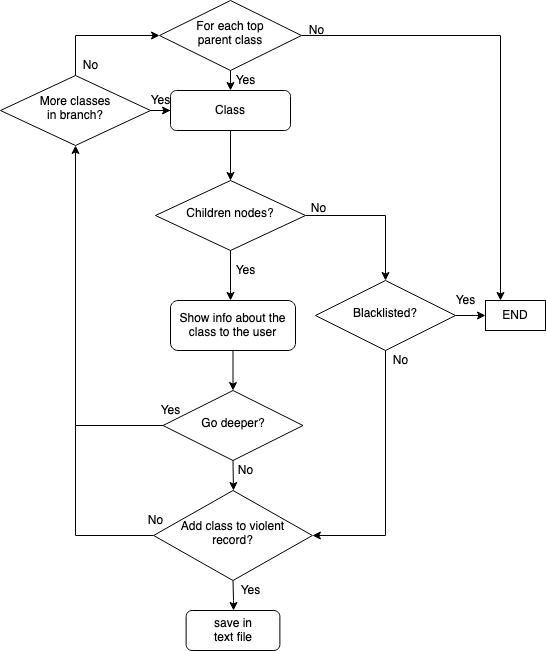
\includegraphics[scale=0.4]{select-vio-cls}
		\caption{Flowchart about selecting violent classes}
		\label{fig:mesh3}
	\end{wrapfigure}
	
	
	Let's say we begin from the class "Human sounds" that is the top level of all sounds emitted by humans contained in the dataset. The system will ask the user if she wants to advance in that direction, i.e., to go across the branches that belong to that part of the tree. If the answer is positive, it would go for the next class, that in this case it would be "Human Speech". It will advance this way until there were no children nodes in the actual class. When this happens, the user will be asked to add the label to the record of \textit{violent classes}, that will be saved in a text file so they can be read by other parts of the model further on. If the user does not want to go deeper, she will be asked to add the current class to the record. If the answer is "No", then they system will jump to the next sibling category. The corresponding flowchart is shown in figure \ref{fig:mesh3}.
	
	This way of flowing through the different classes allows to skip those parts that are not related to our problem. For example, as we can see in figure \ref{fig:mesh1}, one of the top parent labels is "Natural sounds", that relates to sounds from weather phenomena. In most of the cases, these classes will not be selected so the whole branch can be skipped. 

\subsubsection{Downloading videos}

	The following step consists in achieving audio files that belong to the chosen labels. For this purpose, we have made use of the \acrshort{csv} files that were explained in subsection \ref{subsection:data-access}. For each included video, we took its ID and build the corresponding YouTube \acrshort{url}. Once downloaded, we trimmed the file considering the onset and offset and, finally, converted it to audio format (\acrshort{wav}). In our script, we can pass as a parameter the identifier of the desired classes in comma-separated format and either the number of videos per class for a balanced set or a total number of downloads for an unbalanced set. However, there might be some errors when obtaining all the data: the two most common cases are due to lack of enough videos of the desired type in the dataset or because the video is not available anymore on YouTube. When this happens, a message is shown to the user.
	
	It it also worth mentioning that throughout the developing of this downloading task, a script has been coded to achieve the whole dataset in both formats, video and audio, for future works. We are not going to specify anything else since this feature was not finally used.

\subsection{Extracting embeddings}
\label{subsection:extracting-embeddings}

	At this point, all the desired data has been already downloaded to extract the embedded features that will be used to train the model. For this part, we have used the \acrshort{vgg}ish network explained in subsection \ref{subsection:vggish}. Since the audio files duration is usually 10 s, and the embedding extractor gives as a result a vector of size $1 \times 128$ for each second, we will obtain a $10 \times 128$ feature matrix composed by values within the range 0 - 255. Therefore, our input feature matrix will have a size of $(number\ of\ audios) \times 10 \times 128$. The corresponding labels will be stored in a vector of size $(number\ of\ samples)$.
	
	There are some points about the data obtained in this step that should be commented. One of them is about the length of the audio files. As it was previously indicated in \ref{subsection:what-is-audioset}, most of them last 10 s because the creators decided to set this duration for the audio events, but this can change if the video is originally shorter. For these situations, since the model is configured to have an input of $10 \times 128$, the embedding matrix of the shorter clip must be padded with zero-rows to achieve the required dimensions. Even though this does not happen very often, there might be some silent segments that will be labelled with the category of the rest of the audio. A solution for this problem explained later in \ref{section:input-data-preparation} was implemented.
	
	The other case is related to what was explained in \ref{subsection:data-access}. For the recent explanation of how to extract the input features from the audio files we have utilized the first manner of accessing the data, i.e., by reading the \acrshort{csv} files with the videos information before downloading. There is a second option of using the already extracted embedding features. However, these do not look exactly the same when comparing them to the ones obtained by running the \acrshort{vgg}ish with the downloaded videos. This difference is because the implementation of the given code differs from their internal production system in computing issues such as underlying libraries in the installation of \acrshort{vgg}ish and hardware equipment. In spite of this, the result in classification tasks are expected to be equivalent. In order to prove this assumption, we decided to try a small system with both kinds of data. The reason for this check is that although, for this work, the development of the methodologies could be made by using the first and faster manner of accessing the data, for the real implementation in the pendant device within the EMPATIA project (out of our scope) only the second way will be feasible.

\subsection{Assessing the differences between the two types of data access}
\label{subsection:exploring-differences-between-two-types-of-data-access}

	In order to check what is explained above in \ref{subsection:extracting-embeddings}, we have decided to run a little experiment in which a toy classification is performed. Also, we wanted to visualize the different features to check if we could appreciate common patterns by using the \acrfull{tsne} algorithm, which will be explained later in this section.

	Our first step consisted in determining a subset extracted from the original dataset. We thought about choosing for this small application a set composed by three classes that could be considered violent and other three that were non-violent. Apart from this, we paid attention to the number of samples per category to pick some classes over others. Finally, we ended up picking up the labels detailed in table \ref{table:4} and a number of 80 samples for each of them, which led us to a total of 480.
	
	% Table for chosen classes
	\begin{table}[h]
		\begin{center}
			\begin{tabular}{||m{7em} | m{23em} ||}
				\hline
				\textbf{Class} & \textbf{Description} \\
				\hline\hline
				Screaming & A sharp, high-pitched human vocalization; often an instinctive action indicating fear, pain, surprise, joy, anger, etc. Verbal content is absent or overwhelmed, unlike Shout and Yell. \\
				\hline
				Crying, sobbing & Sound associated with the shedding of tears in response to an emotional state, arising from slow but erratic inhalation, occasional instances of breath holding and muscular tremor. \\
				\hline
				Gunshot, gunfire & The sound of the discharge of a firearm, or multiple such discharges. \\
				\hline
				Animal & All sound produced by the bodies and actions of non-human animals. \\
				\hline
				Engine & The sound of a machine designed to produce mechanical energy. Combustion engines burn a fuel to create heat, which then creates a force. Electric motors convert electrical energy into mechanical motion. Other classes of engines include pneumatic motors and clockwork motors. \\
				\hline
				Printer & Sounds of a computer peripheral which makes a persistent human readable representation of graphics or text on paper or similar physical media. \\
				\hline
			\end{tabular}
		\end{center}
		\caption{Chosen classes for a small classification. \textit{Screaming}, \textit{Crying, sobbing} and \textit{Gunshot, gunfire} are considered as the violent ones.}
		\label{table:4}
	\end{table}
	
	For the classification task, we decided to create a small \acrshort{cnn} composed by few layers. Since our input data are matrices of shape $10 \times 128$, these were treated as images so the model was built with layers that perform spatial convolution \cite{Levoy2012}. The architecture is detailed in figure \ref{fig:mesh5}. We used a small kernel size of $3 \times 3$, zero padding so as not to change the shape of the output and a activation of function \acrshort{relu}. Two dense\footnote{Dense is a also a common form to refer to \acrlong{fc} layers. Since each neuron is fed with an input from all the neurons in the previous layer we can say that they are densely connected \cite{Rampurawala2019}} layers are added at the end, first one with also \acrshort{relu} as activation function and the second one with \textit{softmax} to perform the classification, and as many filters as the number of classes.
	
	In order to measure the results, since our subset is balanced, we could have evaluated our model by computing the accuracy and the confusion matrix. More information about these metrics can be found in the appendix \ref{appendix:metrics}. In figure \ref{fig:mesh7}, the four confusion matrices corresponding to the training and test phases for both types of data are shown. Also, in table \ref{table:5}, it is included the accuracy for each case. The results are more accurate when training with the embeddings extracted directly from the audio files we downloaded. When obtaining them from the \acrlong{tf} files, they value of the metrics indicate a worse performance. However, we opted for this second manner because the performance difference is not too big and it requires  much less computational cost and time loss.
	
	% Four confussion matrices
	\begin{figure}[htb]
		% Whole figure
		\captionsetup{justification=centering}
		\begin{subfigure}[b]{\textwidth}
			% Start with figure wav
			\centering
			\captionsetup{justification=centering}
			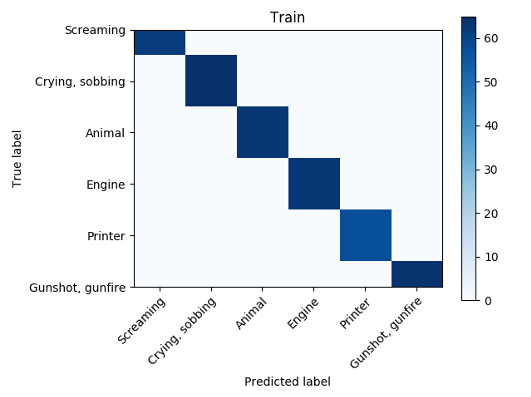
\includegraphics[width=0.5\linewidth]{wav_train}%
			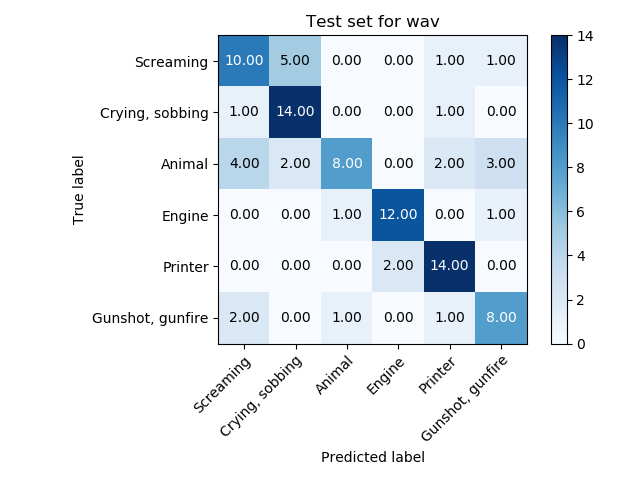
\includegraphics[width=0.5\linewidth]{wav_test}
			\subcaption{Confusion matrices when embeddings are extracted from audio files}
		\end{subfigure}
		\vskip\baselineskip
		% Start with figure tfrecord
		\begin{subfigure}[b]{\textwidth}
			\centering
			\captionsetup{justification=centering}
			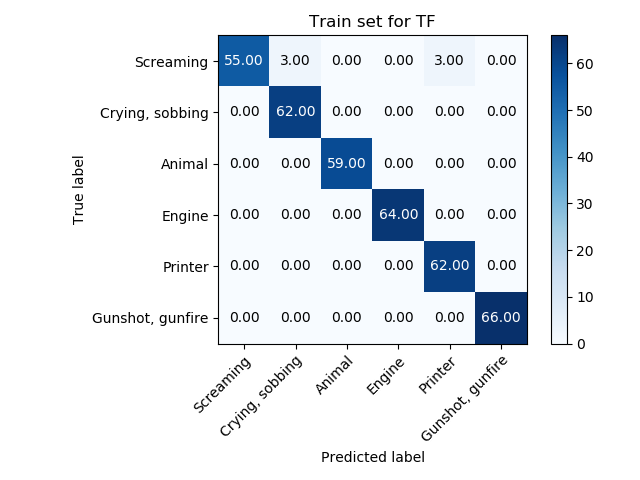
\includegraphics[width=0.5\linewidth]{tfrecord_train}%
			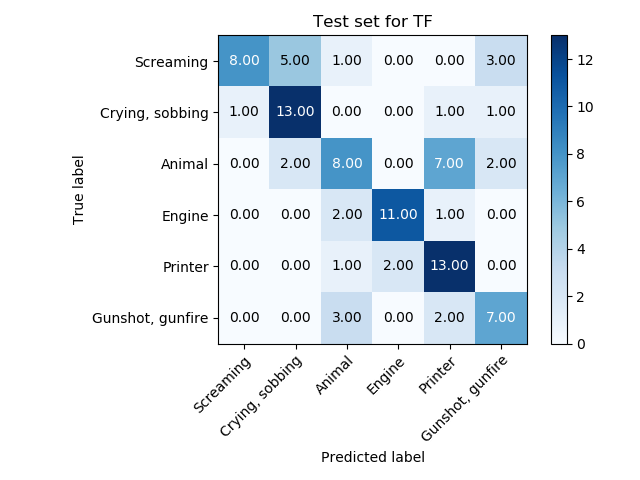
\includegraphics[width=0.5\linewidth]{tfrecord_test}
			\subcaption{Confusion matrices when embeddings are taken from .\textit{tfrecord} files}
		\end{subfigure}
		\caption{Confusion matrices}
		\label{fig:mesh7}
	\end{figure}
	
	% Accuracy values train and test
	\begin{table}[h]
		\begin{center}
			\centering
			\begin{tabular}{|| m{7em} | m{7em} | m{7em} ||}
				\hline
				format / subset & \textbf{Train} & \textbf{Test} \\
				\hline\hline
				\textbf{Audio file} & 0.98 & 0.63 \\
				\hline
				\textbf{.\textit{tfrecord}} & 1.0 & 0.72 \\
				\hline
			\end{tabular}
		\end{center}
		\caption{Accuracy values for audio and .\textit{tfrecord} files}
		\label{table:5}
	\end{table}
	
			% Architecture of model of user interact system
	\begin{wrapfigure}[15]{R}{0.4\textwidth}
		\centering
		\captionsetup{justification=centering}
		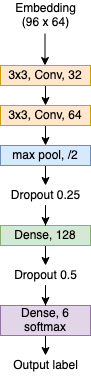
\includegraphics[scale=0.6]{try-wav-tf}
		\caption{Architecture to see how the different embeddings work}
		\label{fig:mesh5}
	\end{wrapfigure}
	
	For the training phases, it can be appreciated that there may be an overfitting since the accuracy is perfect. This means that the \acrshort{nn} stop improving its capacity of learning how to solve the problem in a certain moment of the training task. Instead, it does learn some behaviour pattern that the training data follows. This impacts negatively in the model since the new data that the system will have to learn from will look different and will not follow these same rules \cite{Jabbar2015}. In spite of this result, we did not give it so much importance since we just wanted to do a quick check of the similarity between the two types of data which can be appreciated due to the similarity of both metrics results.
	
\subsubsection{Dimensionality reduction for visualization}
\label{subsection:dimensionality-reduction-for-visualization}

	Apart from the classification exercise, we wanted to see if by plotting the data samples we were able to identify or appreciate some common patterns. In our problem, each of our samples is characterized by a matrix of features with 128 columns, which means that we were working with data belonging to a high-dimensional space. Visualizing this type of data has always been a case of study for many different fields. Plenty of methods have been published so as to find a solution for this task. Some of the most accepted consist on reducing the dimensionality of the data so this can be transformed from the high-dimensional space to a lower one and can be visualize in a common scatter plot of 2D or 3D. These techniques rely on the idea that within a multivariate sample denoted as $x_i = [x_{i1},..., x_{in}]^T$ and considered to be a point that corresponds to a $n-dimensionality$ space, a $d-dimensionality$ space can be found, so that $d < n$. %, in which the data \doubt{is included}. 
	If this is possible, then the observations can be transformed to this lower dimensional space $d$ without any loses \cite{Kaski2011}. 
	
	One of the most common and well-known dimensionality reduction methods is the one known as \acrfull{pca}. This follows the idea previously explained. It specifically aims at extracting the \textit{important} information from the original data and transform them into a set formed by orthogonal variables which are actually known as principal components. This is done by multiplying the matrix data $X$ by a projection matrix $Q$ that contains the coefficients of the linear combinations that allow the conversion. The projections must be orthogonal to each other and they represent the data maximum variance in descending order, being the first component the one with largest variance \cite{Abdi2010}. In fact, each of the projections correspond to an eigenvector in descending order following the value of the eigenvalue. So, the first component will be the eigenvector with the highest eigenvalue. It has been proved to be one of the most appropriated options in dimensionality reduction nowadays. Its use is completely accepted and it is implemented in many famous software libraries. However, it presents some limitations. One of them consists on just considering linear combinations of the original data. When the relation is non-linear, a dimensionality reduction with this technique may result in a loss of information \cite{AmatRodrigo2017}. 
	
	For these cases, other methods have been developed such as \acrfull{tsne}. This algorithm appears as an extension of the previously published \acrfull{sne} \cite{Hinton2003}. Both are based on the same idea of a new way of measuring the similarity between samples. Instead of comparing two observations, let's call them $x_i$ and $y_j$, by computing the euclidean between them, this is done by calculating the conditional probability $p_{j|i}$ of $x_j$ being picked as a neighbour of $x_i$ considering that the samples belong to a Gaussian distribution centered at $x_i$. This depends on how far the samples are from each other, i.e., it is high when they are close and minimum when there are totally separated \cite{VanDerMaaten2008}. Apart from this, two analogous observations are created in the subspace of lower-dimensionality, $y_i$ and $y_j$, and conditional probability $q_{j|i}$ is computed in this situation. It is important that, for $y_i$ and $y_j$ to be faithful representations of $x_i$ and $x_j$, both conditional probabilities must be equal.
	
	In order to calculate the probabilities, a crucial factor is the variance of the Gaussian distribution. There is not a unique valid choice for this parameter, so \acrshort{tsne} performs a binary search so as to find the optimal one \cite{AmatRodrigo2017}. This is also influenced by what is called the perplexity. This can be defined as an assumption of the number of adjacent neighbours for each point. It is a value that is fixed by the user, but it usually belongs to a range from 5 to 50 \cite{VanDerMaaten2008}. 
	
	There are several considerations that should be known before looking at a representation of data from this algorithm \cite{Wattenberg2016}. Actually, it is not an easy task to understand this kind of plots, since the distance between points in the new subspace are not related to the real euclidean distance, which has been denoted as "The Crowding Problem" \cite{VanDerMaaten2008}. This means that the groups cannot be interpreted as real collections of data in the original dimension. However, in order not to misunderstand the data distribution, a couple of visualizations varying the parameters usually tends to be done so that the conclusions can be based on more than one result. In figures \ref{fig:mesh8} and \ref{fig:mesh52}, we show ten \acrshort{tsne} outputs, five for each type of data for diverse values of perplexity from 2 to 50, respectively.
	
	% Four confussion matrices
	\begin{figure}[H]
		% Whole figure
		\captionsetup{justification=centering}
		\begin{subfigure}[b]{\textwidth}
			% Start with figure wav
			\centering
			\captionsetup{justification=centering}
			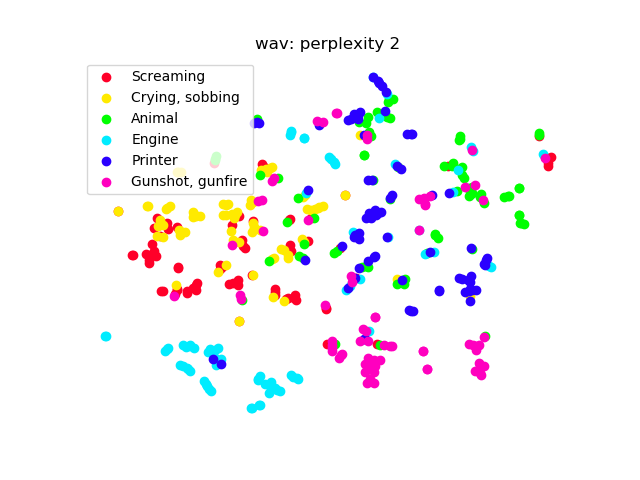
\includegraphics[width=0.5\linewidth]{wav-perp-2}%
			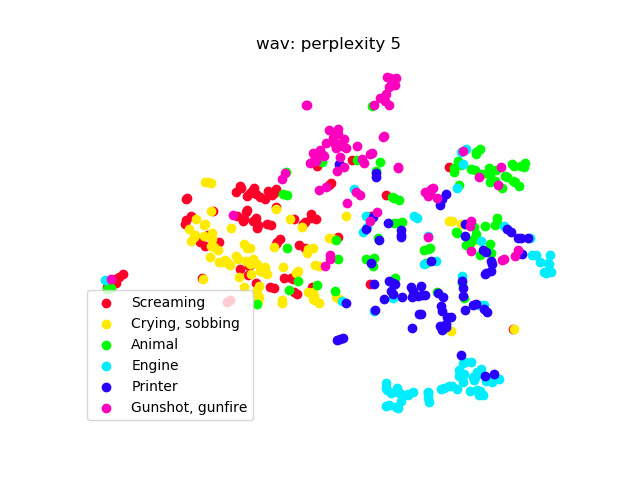
\includegraphics[width=0.5\linewidth]{wav-perp-5}%
		\end{subfigure}
		\vskip\baselineskip
		% Start with figure tfrecord
		\begin{subfigure}[b]{\textwidth}
			\centering
			\captionsetup{justification=centering}
			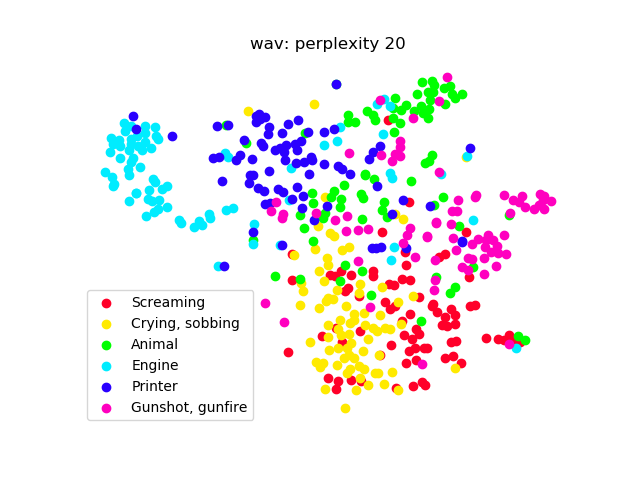
\includegraphics[width=0.5\linewidth]{wav-perp-20}%
			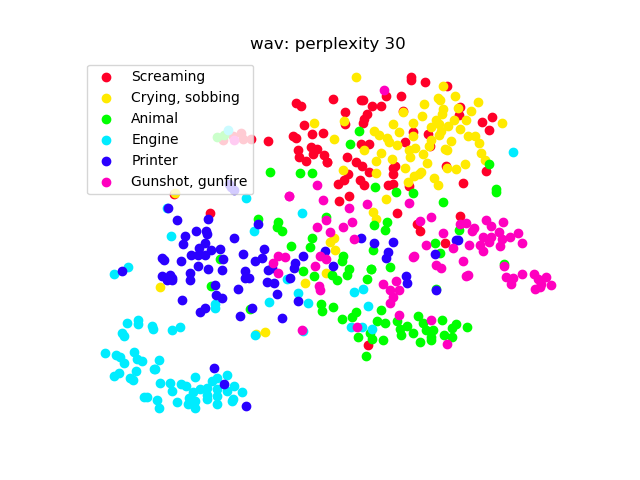
\includegraphics[width=0.5\linewidth]{wav-perp-30}%
		\end{subfigure}
		% 
		\begin{subfigure}[b]{\textwidth}
			\centering
			\captionsetup{justification=centering}
			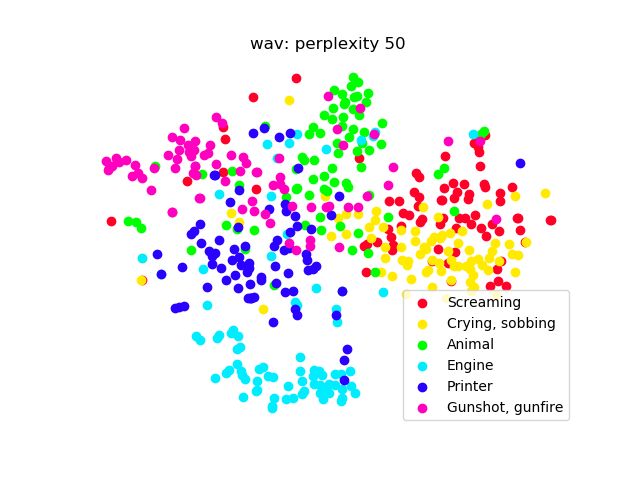
\includegraphics[width=0.5\linewidth]{wav-perp-50}
		\end{subfigure}
		\caption{t-SNE results for wav format with a legend that shows the labels of the corresponding samples in the original 128D space}
		\label{fig:mesh8}
	\end{figure}
	
	\todo{CPM: aumentar las figuras para que se puedan leer las leyendas.}
	
	The selection of the perplexity value depends on the number of observations per class \cite{Wattenberg2016}. Since our subset has 80 samples for each category, we can consider that a proper value is 20 or 30. As we can see, a boundary cannot be extracted among the different labels, but we can see some grouping patterns in the data that correspond to the original labelling and helps us to confirm the similarity of the two different given types. It is true that this method should never be used as an algorithm for clustering itself, but it is a good resource as a backing strategy to other results, as in this case. 
	
	% Four confussion matrices
	\begin{figure}[H]
		% Whole figure
		\captionsetup{justification=centering}
		\begin{subfigure}[b]{\textwidth}
			% Start with figure wav
			\centering
			\captionsetup{justification=centering}
			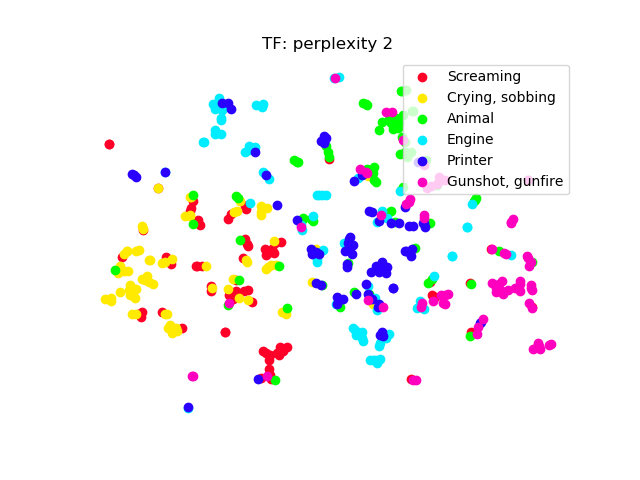
\includegraphics[width=0.5\linewidth]{TF-perp-2}%
			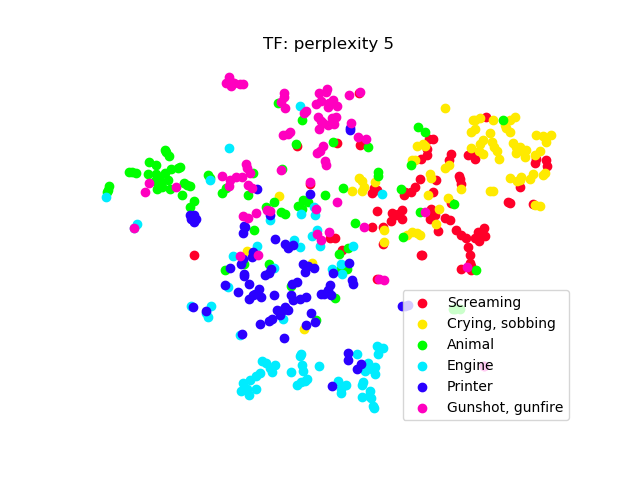
\includegraphics[width=0.5\linewidth]{TF-perp-5}%
		\end{subfigure}
		\vskip\baselineskip
		% Start with figure tfrecord
		\begin{subfigure}[b]{\textwidth}
			\centering
			\captionsetup{justification=centering}
			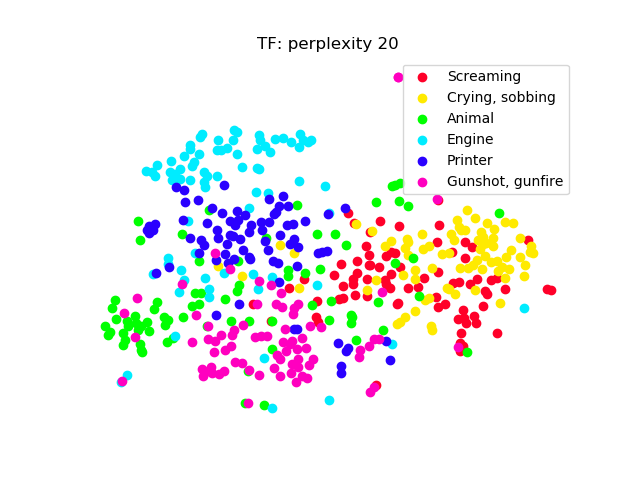
\includegraphics[width=0.5\linewidth]{TF-perp-20}%
			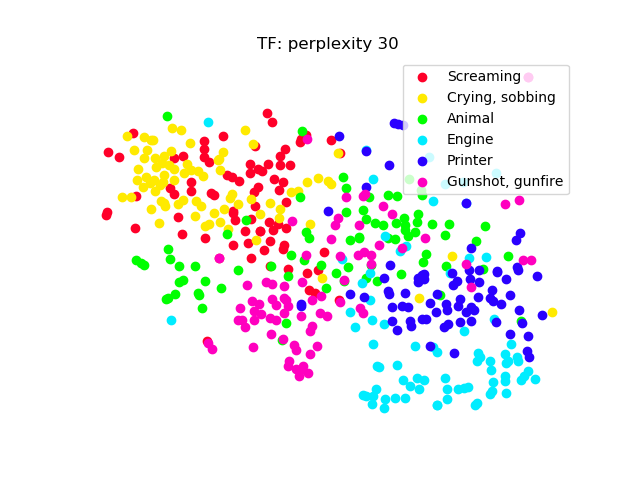
\includegraphics[width=0.5\linewidth]{TF-perp-30}%
		\end{subfigure}
		% 
		\begin{subfigure}[b]{\textwidth}
			\centering
			\captionsetup{justification=centering}
			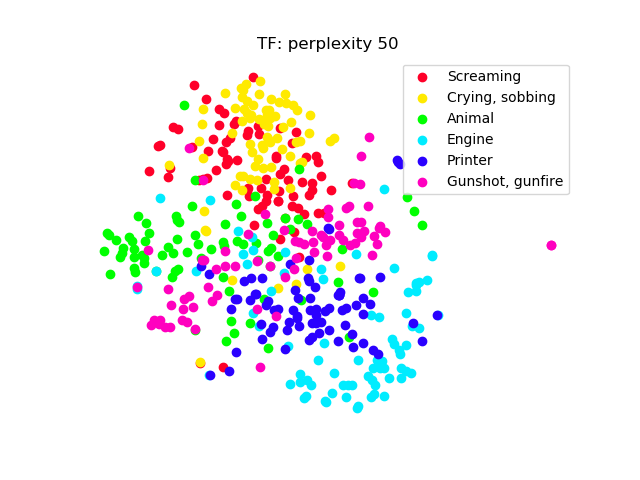
\includegraphics[width=0.5\linewidth]{TF-perp-50}
		\end{subfigure}
		\caption{t-SNE results for .\textit{tfrecord} format with a legend that shows the labels of the corresponding samples in the original 128D space}
		\label{fig:mesh52}
	\end{figure}

\section{Methodology}
\label{section:models}
	
	\todo{Debería poner ejemplos de aplicación al audio como hice en las CNNs o simplemente dejarlo así y ya tratarlo como una parte del estado del arte de related work}
	
% Explain the methods used:
% 1) Data augmentation and SMOTE
% 2) SVM 
% 4) CNN
% 5) LSTM

% !TeX spellcheck = en_GB

\subsection{\acrfull{smote}}
\label{subsection:smote}

	\acrshort{smote} consists of an over-sampling method whose function is to generate synthetic samples in order to populate the minority class in a classification problem by making use of the proper observations that are already contained in the data \cite{Chawla2002}. 
	
	Essentially, this technique works by choosing samples from the minority class that are represented in the features space, placing a line between two of these samples and then select a point inside the line at a random position. First, an arbitrary sample is picked from the minority class and then a number of \textit{k} closest neighbours in the feature space are selected from the same class. One of the neighbours are randomly chosen and a synthetic sample is generated between these two \cite{Browniee2020}. The number of neighbours \textit{k} can vary depending on the amount of over-sampling needed. The value proposed in the publication paper is \textit{k = 5} \cite{Chawla2002}. 
	
	For the generation of the synthetic samples, the distance between the feature vector first arbitrarily selected and one of the nearest neighbours is computed. Then, the resulting value is scaled by multiplying it by a random number that lies in the uniform distribution $U(0,1)$. Finally, this new sample, \textit{S}, is added to the initial feature vector and placed in between these two observations in the feature space \cite{Chawla2002}. \textit{S} can be defined as follows:
	\[S = x + u\cdot(x^{R} - x) \]
	where \textit{x} is the arbitrary selected sample the first time, \textit{u} is the random value from $U(0,1)$ and \textit{x\textsuperscript{R}} is the closest neighbour \cite{Blagus2013}. In figure \ref{fig:mesh47}, it shown a graphical representation of the algorithm. In this case, \textit{X} is the original sample for which the closest neighbours are represented as $X_{i}$, $i=1,2,3,4,5$. The generated samples are $Y_{1}$ and $Y_{2}$ that are place in the line segments.
	
	\begin{figure}
		\centering
		\captionsetup{justification=centering}
		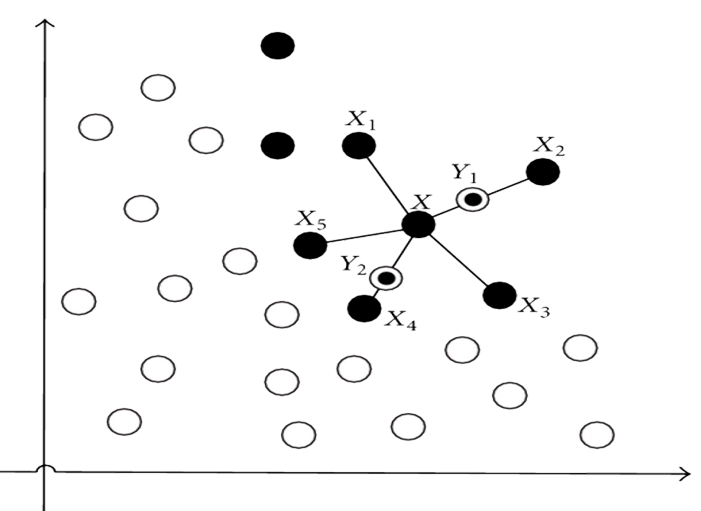
\includegraphics[scale=0.3]{SMOTE}
		\caption{SMOTE algorithm \cite{Xie2015}}
		\label{fig:mesh47}
	\end{figure}

	The common way of applying this technique is in the train set before performing the fit of the model. Usually, an under sampling is performed in the most populated classes and, then, the data augmentation is done for the minority ones \cite{Browniee2020}. Our implementation follows this rule and it is explained in section \ref{section:input-data-preparation}.
	
	 

% !TeX spellcheck = en_GB

\subsection{\acrfull{svm}}
\label{subsection:svm}

	\todo{Adapt...}
	Considering instances of data with their respective ground-truth labels, this classifier finds the frontier defined as a hyperplane that maximizes the distance between the two observations closest to each other that belong to different classes and are more likely to be misclassified. These two points are called support vectors \cite{Fu2011}. This type of method is characterized for being a binary classifier. However, its implementation has been transported to multiclass problems by combining various \acrshort{svm}s in order to stablish a decision criterion so the whole system can chose among $Q$ categories. This can be done by following either one-versus-all or one-versus-one approach. The former addresses the problem training $Q$ classifiers so as to differentiate between data from one class and data from the other $Q-1$ classes. The latter treats the problem by training $Q(Q-1)/2$ \acrshort{svm}s to distinguish among all possible combinations of categories. In any of the approaches, the classification of a certain observation is performed by computing the distance between the sample data and the hyperplane that defines the frontier \cite{Barchiesi2015}. The one-versus-one is the one implemented by \acrfull{svc} from Scikit-learn library and is the one we will use in one of the experiments explained in section \ref{}. In figure \ref{fig:mesh10} it is shown a representation of the decision boundaries that could designed by other type of methods against the hyperplane a \acrshort{svm} classifier would draw.
	
	\begin{figure}[h]
		\centering
		\captionsetup{justification=centering}
		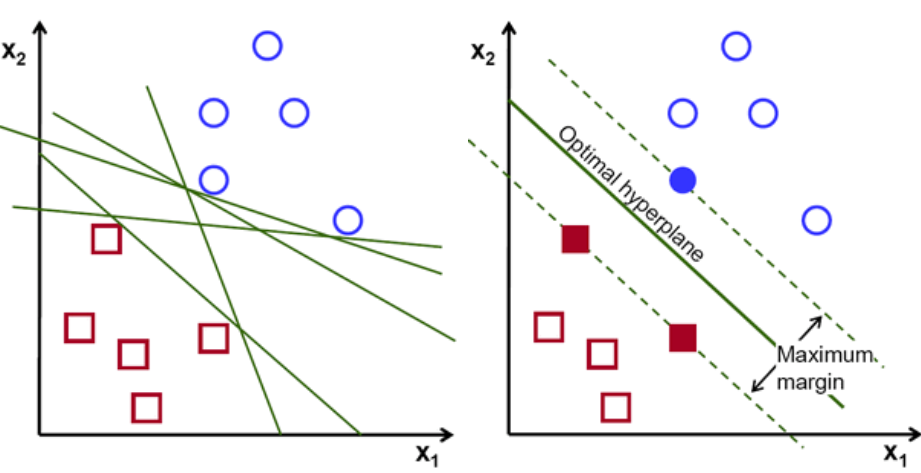
\includegraphics[scale=0.2]{svm}
		\caption{Visualization of a hyperplane set by \acrshort{svm} and other decision boundaries \cite{Drakos2018}}
		\label{fig:mesh10}
	\end{figure}
	
\todo{Add requisites for sklearn algorithm and details about implementation in our model}
\todo{Include definition of kernel and cases}

% !TeX spellcheck = en_GB

\subsection{\acrlong{rnn} and \acrlong{lstm}}

	Human learning does not happen at each moment independently in the sense that every time something new is learned, it depends on the previous knowledge in order to interpret it. This can also be explained by saying that our understanding is persistence.
	
	Traditionally, \acrlong{ann} are not able to act in this way. They \doubt{cannot use the time} as a property to infer conclusions or predictions from the previous instances that belong to a sequence of data. To address this task \acrfull{rnn} have been developed, so they can take information and make it persistent. In figure \ref{fig:mesh39}, it is shown a block of a \acrshort{rnn} in which the network, \textit{A}, is fed with an input \textit{x\textsubscript{t}} that is actually a sequence of data. The output is the value \textit{h\textsubscript{t}}. An inner loop takes the information from the outcome and pass to the input for the next learning step. This can be easily seen in the unrolled part of the right, how the information flows from one element to the next one \cite{Olah2015}. 
	
	\begin{figure}[h]
		\centering
		\captionsetup{justification=centering}
		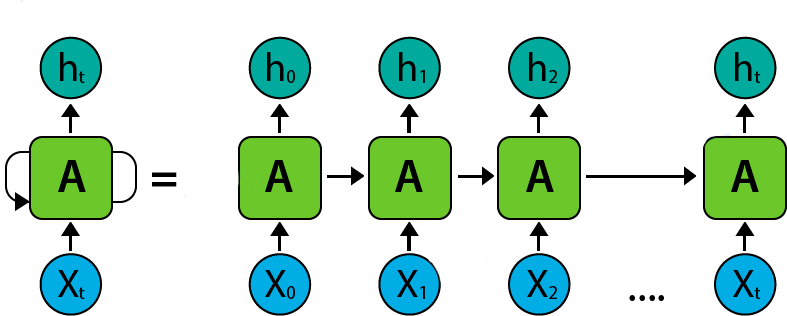
\includegraphics[scale=0.35]{rnn}
		\caption{Scheme or a recurrent neural network about how the loop works }
		\label{fig:mesh39}
	\end{figure}

	This type of networks has became the standard when dealing with sequential data. They have been applied in many tasks, such as language modelling, speech recognition, translation, etc. However, the most simple approach present a problem when the information that must be considering when long-term dependencies. For example, if the task consists of predicting a new instance based on the previous ones in a not really long sequence in which the dependency resides on close instances, normal \acrshort{rnn} can be used and work in the way explained above. When the distance inside the sequence between the predicted element and the ones with the important information that this new one depends on is too large, the network cannot learn this connection \cite{Olah2015}. 
	
	\begin{figure}[h]
		\centering
		\captionsetup{justification=centering}
		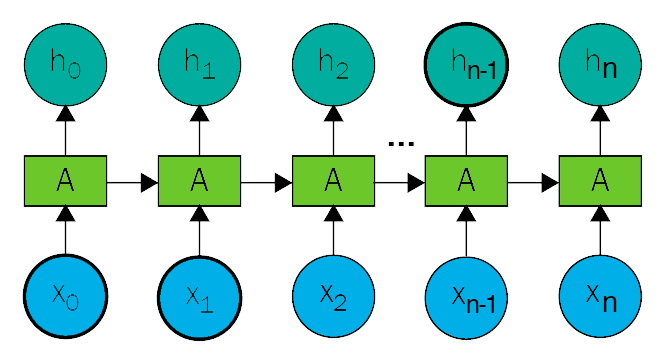
\includegraphics[scale=0.35]{long-term-dependencies}
		\caption{Example of long-term dependencies situation. If the predicted output h\textsubscript{n-1} depends on x\textsubscript{0} and x\textsubscript{1}, the vanishing gradient problem may appear.}
		\label{fig:mesh40}
	\end{figure}
	
	This happens due to the value of the gradients becomes very small during the backpropagation in the learning process. Once the loss function for the new predicted output is calculated, this must be propagated through the rest of the network in order to update the weights. In a typical neural network model, \doubt{the neurons that get updated are those from the hidden layer directly previous to the output one}, but, since the data is a sequence, the neurons from all the earlier layers must be updated as well. The actual problem appears when renovating the value of the weights through time, i.e. updating the weights used to connect the hidden layers in the unrolled temporal loop. So, if the value of the gradient becomes very small the updating process start to be null when finding the new values of the weights and the model stop learning. This is known as the vanishing gradient problem \cite{SuperDataScienceTeam2018}.
	
	As a solution, a new type of \acrshort{rnn} was developed and named as \acrfull{lstm} networks. These can be defined as a recurrent network that can learn long-term dependencies, so the vanishing gradient problem is not an issue for these models. Nowadays, they are widely used in several fields, since they can remember information along long periods \cite{Olah2015}. The main structure along is the same shown above in figure \ref{fig:mesh39}. The difference from the way of working in a common \acrshort{rnn} is the inner architecture in the neural network. In \acrshort{lstm}, the \textit{A} modules are defined as shown in figure \ref{fig:mesh41}. The notation used is as follows: the rectangles denotes a neural network layer, the circle shapes refer to point-wise operations and the arrows means vector transferring.
	
	\begin{figure}
		\centering
		\captionsetup{justification=centering}
		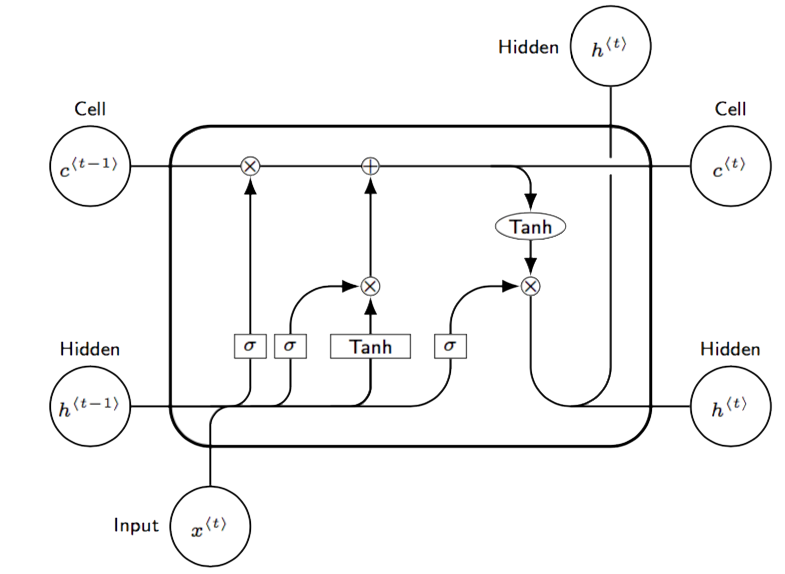
\includegraphics[scale=0.29]{lstm-module}
		\caption{LSTM module with the representation of the different operations that take place inside of it}
		\label{fig:mesh41}
	\end{figure}

	The main concept of a \acrshort{lstm} network resides on its cell state and the different gates. The cell state, represented in the diagram by the upper arrow, is the one in charge of transferring information all the way through the chain of modules. It can be thought as the memory of the whole network. Its objective is to just carry information considered relevant for the model. This way is how the \acrshort{lstm} brings the information from the first layers to the last ones without suffering the vanishing gradient problem. The content of the cell state is modified by the point-wise operations that acts by following the gates criteria. These are in fact neural networks that has the goal of deciding which information can be treated as relevant and so added to cell state. This process can be understood as a learning/forgetting stage \cite{Nguyen2018}. 
	
	In order to understanding how this process works, we are going the interaction of the different gates in the learning stage.

	\begin{wrapfigure}{l}{0.26\textwidth}
		\centering
		\captionsetup{justification=centering}
		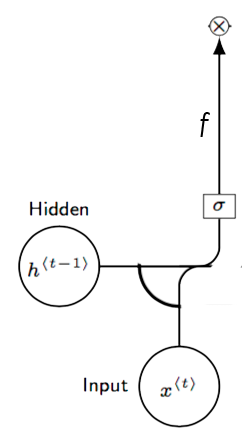
\includegraphics[scale=0.25]{lstm-forget-gate}
		\caption{Step 1. Forget gate}
		\label{fig:mesh42}
	\end{wrapfigure}

	The first step is performed by what is called the \textit{forget gate} layer. It must decide which information must be included in the cell state that travels through the time chain. This is way the layer contains a sigmoid function that outputs values between  0 and 1, in which  0 means dropping the information in the previous cell state and 1 implies to keep it. As shown in figure \ref{fig:mesh42}, this is done by paying attention to the hidden state which is the output of the previous module, \textit{h\textsuperscript{<t-1>}}, and the input of the current one, \textit{x\textsuperscript{<t>}} \cite{Nguyen2018}. The resulting function $f$ is defined as follows, where $W_{f}$ are the weights of the \acrshort{rnn} and $b_{f}$ the bias.
	\[
	\ f = \sigma(W_{f}[h^{t-1}, x^{t}] + b_{f})
	\]
	
	\begin{wrapfigure}{r}{0.3\textwidth}
		\centering
		\captionsetup{justification=centering}
		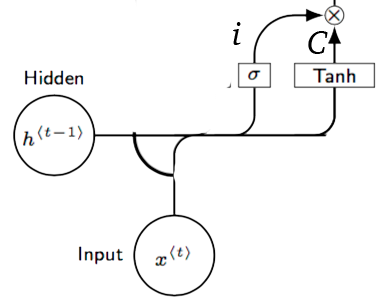
\includegraphics[scale=0.27]{lstm-input-gate}
		\caption{Step 2. Input gate}
		\label{fig:mesh43}
	\end{wrapfigure}
	
	Next, the decision about what information from the current input \textit{x\textsuperscript{<t>}} must be taken to the cell state is performed. The gate that computes this operation receives the name of \textit{input gate}. This part can be divided into two different steps. First, the previous hidden state,\textit{x\textsuperscript{<t-1>}} ,and the current input feed a \acrshort{rnn} with a sigmoid for the activation function, which takes the decision of \doubt{which values must be updated} by converting them into a range limited by 0 and 1. This result denotes the importance of the value, being 0 non-important and 1, important. Then, also \textit{h\textsuperscript{<t-1>}} and \textit{x\textsuperscript{<t>}} are used as input for the \acrshort{tanh} layer so the values are mapped between -1 and 1. This last activation function is included in order to \doubt{avoid the vanishing gradient problem previously mentioned, since a function whose second derivative takes more time to tend to zero is needed}. Finally, both outputs are multiplied before the updating process in the cell state \cite{Nguyen2018}. The equations for the output of each \acrshort{rnn} module are included below, where $W$ and $b$ denotes the weights and bias for each layer \cite{Olah2015}.
	\[ i = \sigma(W_{i}[h^{t-1}, x^{t}] + b_{i}) \]
	\[ C = \tanh(W_{C}[h^{t-1}, x^{t}] + b_{C}) \]
	
	In the step 3, the output of the multiplication from the input gate layer and the output $f$ of the sigmoid function from the forget gate, modify the old cell state from the previous module, \textit{c\textsuperscript{<t-1>}}, so it can be updated. For the outcome of the step 1, a point-wise multiplication is performed, $f * C^{<t-1>}$. Then, to the output of this operation is added the resulting product of the input gate, $i * C$. This two operations can be translated as a forgetting and a learning stage. First, the values the forget gate decided to remove from the cell state are actually forgotten. Then, it must learn the new values belonging to the current input also weighted by their importance, what denotes how much the state values are going to be updated \cite{Olah2015}. The new cell state expression $c^{t}$ is included below and the process is shown in figure \ref{fig:mesh44}.
	
	\begin{wrapfigure}{l}{0.4\textwidth}
		\centering
		\captionsetup{justification=centering}
		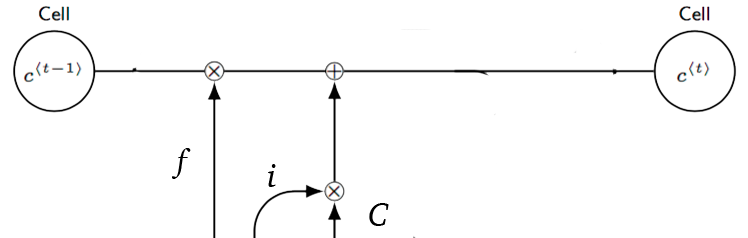
\includegraphics[width=\linewidth]{lstm-cell-state}
		\vspace{-10pt}
		\caption{Step 3. Update cell state}
		\label{fig:mesh44}
	\end{wrapfigure}
	
	
	\[c^{<t>} = f * C^{<t-1>} + i * C\]
	
				
	Finally, the last step of the module corresponds to the \textit{output gate}. This has the function of deciding how the next hidden state is going to be like. First, \textit{x\textsuperscript{<t>}} and \textit{h\textsuperscript{<t-1>}} are used as input for a layer with a sigmoid activation function and the output $o$ is obtained. Also, the cell state \textit{c\textsuperscript{<t>}} feeds a point-wise \acrshort{tanh} so its values are clipped between -1 and 1. Both outputs are multiplied. The $o$ result decides what values form the current input must be kept in the future hidden state,\textit{h\textsuperscript{<t>}}. The actual output of the module is the hidden state. It also transports the relevant information updated together with the cell state to the next network. The outputs $o$ and $h^{t}$ can be defined as shown below. Also, in figure \ref{fig:mesh45}, the stage of this last part is included.
		
	\begin{figure}{h}
		\centering
		\captionsetup{justification=centering}
		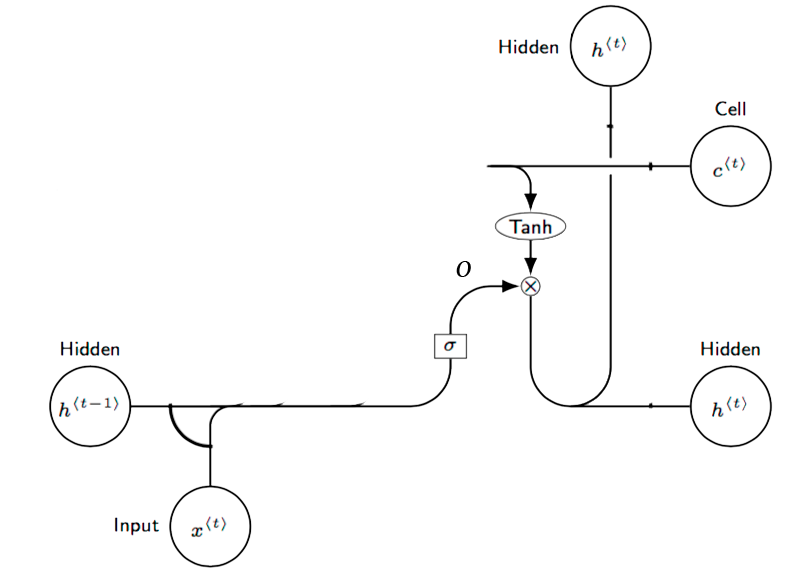
\includegraphics[scale=0.25]{lstm-output-gate}
		\caption{Step 3. Output gate}
		\label{fig:mesh45}
	\end{figure}
	
	\[ o = \sigma(W_{o}[h^{<t-1>, x^{t}}] + b_{o}) \]
	\[ h^{<t>} = o * \tanh(C) \]
	
	
	
	






















